%Afsnit 3 analyserer vi problemet (oversættelsen fra Hermes uden sidekanaler til ARM).
%Hvordan gør vi det egentlig, hvad skal vi være opmærksom på:
%Værktøjer vi bruger, hvorfor bruger vi dem, hvad skal vi gøre for at de kan bruges.
%Når afsnit 3 er færdig, så ved læseren hvad man skal gøre.
In our compilation from Hermes to ARM64 using Moscow ML\footnote{Moscow ML is a functional programming language widely used for teaching and research. More can be found at \url{http://www.itu.dk/~sestoft/mosml.html}}, we need to be aware of several things.

We are skipping some steps, as the current implementation is from Hermes to C and then to ARM.
But by skipping these steps, we have an easier time analyzing and optimizing. The question is how do we do it and what do we need to consider?

\section{Grammar}
In Figure \ref{fig:hermes_grammar} the Hermes grammar is presented.
A Hermes Program consists of one or more Hermes Procedures each with an \bf{id}, a potentially empty list of declarations (function parameters) and a Hermes Block statement consisting of zero or more Hermes Stmts.
One of these Procedures must have the \bf{id} \emph{main} and take no arguments. This is the procedure that is first called when the program is executed.
Every procedure has to have exactly one Block statement. A Block is a special statement corresponding to a function body, consisting of a list of variable declarations followed by a list of Hermes Stmts.
Variable declarations (\emph{Decls1}) can be either variables, dynamic arrays or constants. Constants and constant arrays are public types are therefore not required to be zero at the end of a function. It is the responsibility of the programmer to make sure that sensitive information gets stored in the right variables.
Prior to this thesis Hermes only allowed constant declarations to be variables, but this has been extended allow constant matrix declarations as well.
A ConstArrayDecl in the abstract syntax tree has the type \bf{string * string * string list * typ * pos} which corresponds to name, size, elements, type and position.
\begin{figure}[htp]
\centering
\begin{tabular}{>{$}l<{$}>{$}r<{$}>{$}l<{$}}
    Program   & \rightarrow & Procedure^+ \\[7pt]
    Procedure & \rightarrow & \textbf{id} \; ( \; Decls2^? \; ) \; Stmt \\[7pt]
    Stmt      & \rightarrow &; \\
              & |           & Lval \; \textbf{update} \; Exp \;; \\
              & |           & Lval\text{++} \;; \\
              & |           & Lval\text{- -} \;; \\
              & |           & \texttt{if} \; ( \; Exp \; ) \; Lval \; \textbf{update} \; Exp \;; \\
              & |           & Lval \; \text{<->} \; Lval \;; \\
              & |           & \texttt{if} \; ( \; Exp \; ) \; Lval \; \text{<->} \; Exp \;; \\
              & |           & \texttt{for} \; ( \; \textbf{id} = Exp \; ; \; Exp \; ) \; Stmt  \;; \\
              & |           & \texttt{assert} \; ( \; Exp \; ) \;; \\
              & |           & \texttt{call} \; \textbf{id} \; ( \; Lvals \; ) \;; \\
              & |           & \texttt{uncall} \; \textbf{id} \; ( \; Lvals \; ) \;; \\
              & |           & \texttt{printf} \; ( \; \textbf{stringConst} \; , \; Lvals \; ) \;; \\
              & |           & \texttt{scanf} \; ( \; \textbf{stringConst} \; , \; Lvals \; ) \;; \\
              & |           & \{ \; Decls1 \; Stmt^* \; \} \\[7pt]
    Exp       & \rightarrow & Lval \\
              & |           & \textbf{numConst} \; \\
              & |           & Exp \; \textbf{binOp} \; Exp \\
              & |           & \textbf{unOp} \; Exp \\
              & |           & ( \; Exp \; ) \; \\[7pt]
    Lval      & \rightarrow & \textbf{id}\\
              & |           & \textbf{id} \; [ \; Exp \; ] \\[7pt]
    Lvals     & \rightarrow & Lval \\
              & |           & Lval \; , \; Lvals \\[7pt]
    VarSpec   & \rightarrow & \textbf{id}\\
              & |           & \textbf{id} \; [ \; \textbf{numConst} \; ] \\[7pt]
    VarSpecs  & \rightarrow & VarSpec \\
              & |           & VarSpec \; , \; VarSpecs \\[7pt]
    Decls1    & \rightarrow & \\
              & |           & \textbf{type} \; Varspecs \; ; \; Decls1\\
              & |           & \texttt{const}\;\textbf{type}\;\textbf{id}\;=\textbf{numConst}\;;\;Decls1\;\\[7pt]
    Decls2    & \rightarrow & \textbf{type} \; VarSpec \\
              & |           &  \textbf{type} \; VarSpec \; , \; Decls2

\end{tabular}
\caption{Grammar of Hermes.}
\label{fig: grammar}
\end{figure}



\clearpage
\newpage

\section{Intermediate representations}
When compiling Hermes to RSSA, we use the procedure introduced in Section~\ref{section - RIL}.
We can do this in two iterations: first we translate to RIL, and then we translate to RSSA.
The reason for doing it in two steps is to postpone the problem of register allocation, and keep the two problems seperated.
We will be creating an abstract syntax tree that RIL and RSSA will share.
As seen in Figure~\ref{fig:RIL vs RSSA}, the main difference between the two representations is the subscript index on the left-values.
% TODO: omskriv til egen tabel. Det ser alt for grynet ud med det billede der.
\begin{table}[htp]
  \centering
  \begin{tabular}{| a | b |}
    \hline
    RIL                             & RSSA                            \\ \hline
    $x\ \ \oplus= R_1 \odot R_2$    & $x_i := x \oplus R_1 \odot R_2$ \\ \hline
    $M[x]\ \oplus= R_1 \odot R_2$   & $M[x] \oplus= R_1 \odot R_2$    \\ \hline
    $x \leftrightarrow y$           & $x_i, y_j := y, x$              \\ \hline
    $M[x] \leftrightarrow M[y]$     & $M[x] \leftrightarrow M[y]$     \\ \hline
    $x \leftrightarrow M[y]$        & $x_i := M[y] := x$              \\ \hline
    $M[y] \leftrightarrow x$        & $x_i := M[y] := x$              \\ \hline
    call $l$                        & $() := \text{call  } l()$       \\ \hline
    uncall $l$                      & $() := \text{uncall  } l()$     \\ \hline
  \end{tabular}
  \caption[caption]{RIL and RSSA syntax from\cite{10.1007/978-3-319-41579-6_16}.}
  \label{fig:RIL vs RSSA}
\end{table} \\
%\begin{figure}[htp]
%  \begin{center}
%    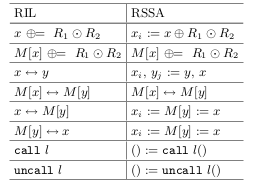
\includegraphics[width=0.6\textwidth]{RIL_RSSA_syntax.png}
%  \end{center}
%  \caption[caption]{RIL and RSSA syntax from\cite{10.1007/978-3-319-41579-6_16}.}
%  \label{fig:RIL vs RSSA}
%\end{figure} \\
Variables that are going to have an index can be represented in SML as a tuple of a string variable name and an integer option index. The integer option can be NONE in the first iteration to RIL, and SOME int in the second iteration to RSSA. This makes it easy to seperate the two tasks and handle the indexing once the program has already been transformed to RIL.

Table~\ref{table:translation} shows the correlation between Hermes statements and RSSA statements. Keep in mind that block, printf, scanf and assertion statements do not result in anything as they are only for debugging Hermes.
\begin{table}[htp]
  \begin{tabular}{| a | b |}
    \hline
    Hermes              & RSSA                          \\ \hline
    Hermes.Skip         & RSSA.Skip                     \\ \hline
    Hermes.Update       & RSSA.Assign / RSSA.MemUpdate  \\ \hline
    Hermes.CondUpdate   & RSSA.If                       \\ \hline
    Hermes.Inc          & RSSA.Assign / RSSA.MemUpdate  \\ \hline
    Hermes.Dec          & RSSA.Assign / RSSA.MemUpdate  \\ \hline
    Hermes.Swap         & RSSA.AssignSwap / RSSA.MemSwap / RSSA.VarMemSwap \\ \hline
    Hermes.CondSwap     & RSSA.If with translated swap inside body \\ \hline
    Hermes.For          & RSSA.For  \\ \hline
    Hermes.Call         & RSSA.Call \\ \hline
    Hermes.Uncall       & RSSA.Uncall \\ \hline
  \end{tabular}
  \caption{Translation table from Hermes to RSSA.}
  \label{table:translation}
\end{table}

\clearpage
\newpage

\section{Translation example}
In the following example we will look at a Hermes program that increments a variable and performs an update with addition.
Usually it will be the programmers task to ensure a functions local values are zeroed out before the end of the function. However, to simplify  things we will omit this in the following translation example.

After the parser and the lexer has run, as shown in Listing~\ref{listing:handtranslateHermesInternal}, the internal Hermes representation has the name of the function we are defining ``main``, followed by an empty list of decls i.e. the function parameters.
Then follows the function body as a Block statement with local variable declarations and a list of statements corresponding to the ``\lstinline{++}`` and ``\lstinline{+=}`` statements in Listing~\ref{listing:handtranslateHermes}.

When the RSSA compiler has run, as shown in Listing~\ref{listing:handtranslateRSSAInternal}, the internal Hermes representation has been transformed into an internal RSSA representation containing references to variables and arrays etc.
As there are no RSSA statements for declaring variables, declarations are handled separately as shown in Listing~\ref{listing:handtranslateRSSA}. They are translated to initialization- and finalization-strings in accordance to the RSSA standard from\cite{10.1007/978-3-319-41579-6_16} and inserted by the pretty-printer in case the target language is RIL or RSSA.

When the ARM compiler has run, as shown in Listing~\ref{listing:handtranslateARMInternal}, the internal RSSA representation has been transformed into an internal ARM representation.
As the internal representation of ARM is just a list of instructions, the pretty-printer just prints out the instructions as shown in Listing~\ref{listing:handtranslateARM} and does a little formatting. Rotate left (ROL) becomes rotate right as discussed earlier.

\lstinputlisting[label=listing:handtranslateHermes, caption=Here we see an example of a simple Hermes program that does addition., language=Hermes, float=tp]{"Listings/handtranslateHermes.hms"}

\lstinputlisting[label=listing:handtranslateHermesInternal, caption=Here we see the Hermes internal representation of Listing~\ref{listing:handtranslateHermes}., language=Hermes, float=tp]{"Listings/handtranslateHermesInternal"}

\lstinputlisting[label=listing:handtranslateRSSAInternal, caption=Here we see the RSSA internal representation of Listing~\ref{listing:handtranslateHermes}., language=Hermes, float=tp]{"Listings/handtranslateRSSAInternal"}


\lstinputlisting[label=listing:handtranslateRSSA, caption=Here we see the pretty-printed version of the RSSA internal representation of Listing~\ref{listing:handtranslateRSSAInternal}., float=tp]{"Listings/handtranslateRSSA"}

\lstinputlisting[label=listing:handtranslateARMInternal, caption=Here we see the ARM internal representation of Listing~\ref{listing:handtranslateHermes}., language=Hermes, float=tp]{"Listings/handtranslateARMInternal"}

\lstinputlisting[label=listing:handtranslateARM, caption=Here we see the pretty-printed version of the ARM internal representation of Listing~\ref{listing:handtranslateARMInternal}., language=Hermes, float=tp]{"Listings/handtranslateARM"}

\clearpage
\newpage

\section{Protection from side-channels}
A key part of our compilation is to protect against side-channel attacks.
Hermes guarantees that no sensitive information will be left in memory after execution, but what about after translation to RSSA and ARM64?
As discussed earlier, RSSA has been developed in such a way that every variable has an initialization and finalization.
The ARM64 implementation currently has abstract register names.
Once added, it would be the job of a register allocator to handle initialization and finalization.
With regards to timing attacks Hermes has two control structures: conditional swaps and conditional updates.
Both contain only one line of code to be executed and remain semantically equivalent in RSSA and ARM64.

Some hardware architectures do not have constant time multiplication and division.
The modulo operation can also be vulnerable, if it has been implemented using multiplication and division.
One of the most commonly used techniques for modulo is called Barrett Reduction\cite{mod_without_mod} where the general idea is
\begin{equation*}
  X \text{ mod } Y \equiv X - \lfloor{ X / Y }\rfloor Y
\end{equation*}
Here X is divided by Y, floored, and then multiplied with Y. The resulting value is the closest multiple of Y to X. That value is then subtracted from X to give the modulo. 
Fortunately it seems ARM architectures beginning with ARM9E have constant time multiplication and division\cite{bearssl}.
It is still something to keep in mind, however, should we wish to extend Hermes with another target assembly language in the future.
